% Editable textbook TikZ, initially imported from the verified semantic plate.
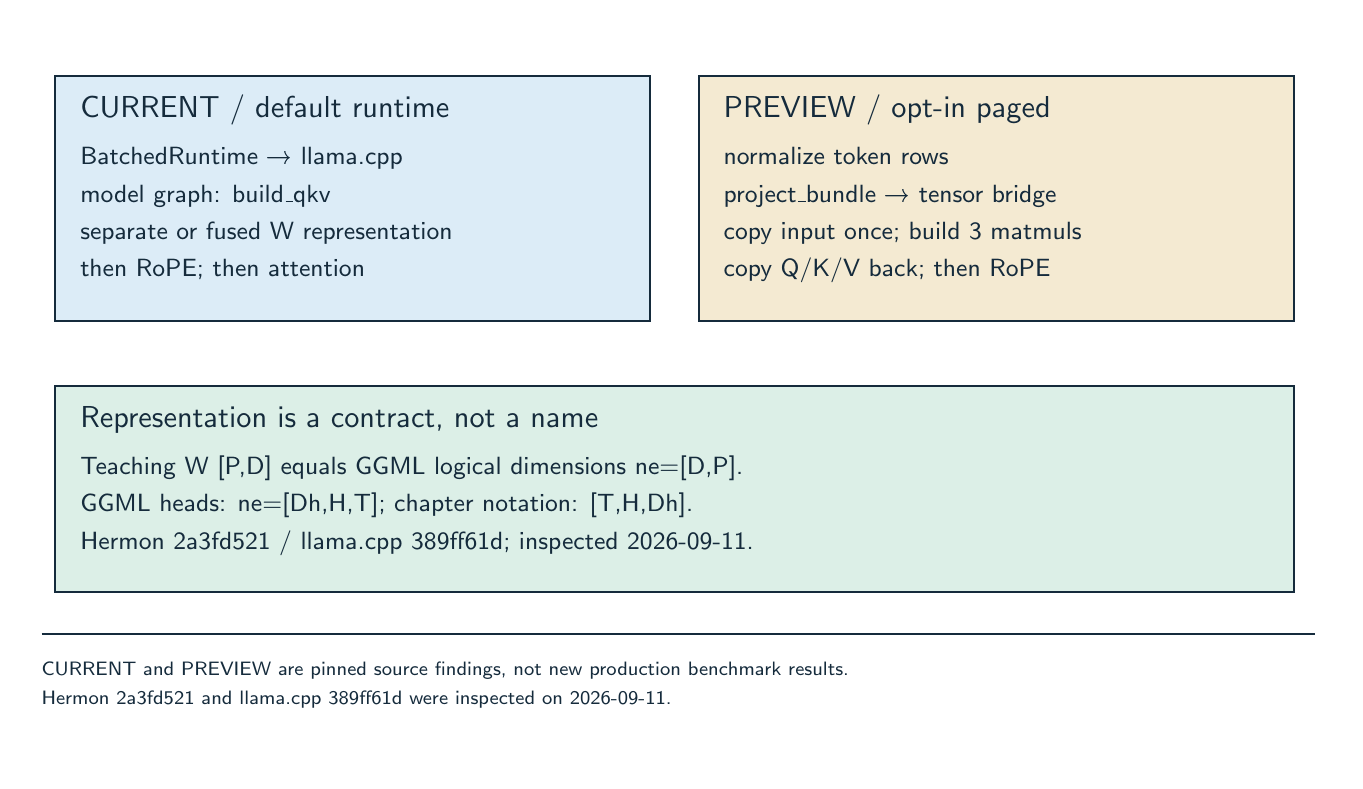
\begin{tikzpicture}[x=.5pt,y=-.5pt]
\path[use as bounding box] (30,170) rectangle (975,700);
\path[fill={rgb,255:red,220;green,236;blue,247},draw={rgb,255:red,21;green,43;blue,60},line width=0.7pt] (50.0,205.0) rectangle (480.0,382.0);
\node[inner sep=0pt,outer sep=0pt,anchor=base west,text={rgb,255:red,21;green,43;blue,60},font=\sffamily\fontsize{9.5}{11.4}\selectfont] at (64,234) {};
\node[inner sep=0pt,outer sep=0pt,anchor=base west,text={rgb,255:red,21;green,43;blue,60},font=\sffamily\fontsize{10.5}{12.6}\selectfont] at (68,235) {CURRENT / default runtime};
\node[inner sep=0pt,outer sep=0pt,anchor=base west,text={rgb,255:red,21;green,43;blue,60},font=\sffamily\fontsize{9.0}{10.799999999999999}\selectfont] at (68,269) {BatchedRuntime → llama.cpp};
\node[inner sep=0pt,outer sep=0pt,anchor=base west,text={rgb,255:red,21;green,43;blue,60},font=\sffamily\fontsize{9.0}{10.799999999999999}\selectfont] at (68,296) {model graph: build\_qkv};
\node[inner sep=0pt,outer sep=0pt,anchor=base west,text={rgb,255:red,21;green,43;blue,60},font=\sffamily\fontsize{9.0}{10.799999999999999}\selectfont] at (68,323) {separate or fused W representation};
\node[inner sep=0pt,outer sep=0pt,anchor=base west,text={rgb,255:red,21;green,43;blue,60},font=\sffamily\fontsize{9.0}{10.799999999999999}\selectfont] at (68,350) {then RoPE; then attention};
\path[fill={rgb,255:red,244;green,234;blue,210},draw={rgb,255:red,21;green,43;blue,60},line width=0.7pt] (515.0,205.0) rectangle (945.0,382.0);
\node[inner sep=0pt,outer sep=0pt,anchor=base west,text={rgb,255:red,21;green,43;blue,60},font=\sffamily\fontsize{9.5}{11.4}\selectfont] at (529,234) {};
\node[inner sep=0pt,outer sep=0pt,anchor=base west,text={rgb,255:red,21;green,43;blue,60},font=\sffamily\fontsize{10.5}{12.6}\selectfont] at (533,235) {PREVIEW / opt-in paged};
\node[inner sep=0pt,outer sep=0pt,anchor=base west,text={rgb,255:red,21;green,43;blue,60},font=\sffamily\fontsize{9.0}{10.799999999999999}\selectfont] at (533,269) {normalize token rows};
\node[inner sep=0pt,outer sep=0pt,anchor=base west,text={rgb,255:red,21;green,43;blue,60},font=\sffamily\fontsize{9.0}{10.799999999999999}\selectfont] at (533,296) {project\_bundle → tensor bridge};
\node[inner sep=0pt,outer sep=0pt,anchor=base west,text={rgb,255:red,21;green,43;blue,60},font=\sffamily\fontsize{9.0}{10.799999999999999}\selectfont] at (533,323) {copy input once; build 3 matmuls};
\node[inner sep=0pt,outer sep=0pt,anchor=base west,text={rgb,255:red,21;green,43;blue,60},font=\sffamily\fontsize{9.0}{10.799999999999999}\selectfont] at (533,350) {copy Q/K/V back; then RoPE};
\path[fill={rgb,255:red,220;green,239;blue,231},draw={rgb,255:red,21;green,43;blue,60},line width=0.7pt] (50.0,429.0) rectangle (945.0,578.0);
\node[inner sep=0pt,outer sep=0pt,anchor=base west,text={rgb,255:red,21;green,43;blue,60},font=\sffamily\fontsize{9.5}{11.4}\selectfont] at (64,458) {};
\node[inner sep=0pt,outer sep=0pt,anchor=base west,text={rgb,255:red,21;green,43;blue,60},font=\sffamily\fontsize{10.5}{12.6}\selectfont] at (68,459) {Representation is a contract, not a name};
\node[inner sep=0pt,outer sep=0pt,anchor=base west,text={rgb,255:red,21;green,43;blue,60},font=\sffamily\fontsize{9.0}{10.799999999999999}\selectfont] at (68,493) {Teaching W [P,D] equals GGML logical dimensions ne=[D,P].};
\node[inner sep=0pt,outer sep=0pt,anchor=base west,text={rgb,255:red,21;green,43;blue,60},font=\sffamily\fontsize{9.0}{10.799999999999999}\selectfont] at (68,520) {GGML heads: ne=[Dh,H,T]; chapter notation: [T,H,Dh].};
\node[inner sep=0pt,outer sep=0pt,anchor=base west,text={rgb,255:red,21;green,43;blue,60},font=\sffamily\fontsize{9.0}{10.799999999999999}\selectfont] at (68,547) {Hermon 2a3fd521 / llama.cpp 389ff61d; inspected 2026-09-11.};
\draw[fill=none,draw={rgb,255:red,21;green,43;blue,60},line width=0.75pt] (40,608) -- (960,608);
\node[inner sep=0pt,outer sep=0pt,anchor=base west,text={rgb,255:red,21;green,43;blue,60},font=\sffamily\fontsize{7.5}{9.0}\selectfont] at (40,638) {CURRENT and PREVIEW are pinned source findings, not new production benchmark results.};
\node[inner sep=0pt,outer sep=0pt,anchor=base west,text={rgb,255:red,21;green,43;blue,60},font=\sffamily\fontsize{7.5}{9.0}\selectfont] at (40,659) {Hermon 2a3fd521 and llama.cpp 389ff61d were inspected on 2026-09-11.};
\end{tikzpicture}
